\documentclass[10pt,a4paper,onecolumn]{report}
\usepackage[latin1]{inputenc}
\usepackage{amsmath}
\usepackage{amsfonts}
\usepackage{amssymb}
\usepackage{listings}
\usepackage{courier}
\usepackage{array}
\usepackage{graphicx}
\usepackage[margin=1in]{geometry}
\author{Moataz Elmasry and Monica Paun}
\title{Advanced Vision Assignment 1}

\begin{document}
\lstset{language=Matlab} 

\maketitle

\begin{abstract}

In this report, we outline our attempt at identifying and tracking a set of marbles moving across a fixed featureless background. The first section of the report discusses the detection of the marbles in each individual frame, the second section discusses the tracking of the marbles across consecutive frames. For each of the tasks, we describe the algorithm used, and its performance.

\end{abstract}

\chapter{Marble Detection}

\section{Algorithm}

\subsection{Object-oriented Approach}

Given the large number of unique dynamic marbles that need to be identified and the apparent complexity of information represented by every image frame, we decided to use an object-oriented approach to better tackle the assignment. Despite adding an extra overhead in terms of coding effort, this approach proved very beneficial with regards to understanding, maintaining and structuring the code.

Image objects were represented by such things as their number in the dataset, their connected components, and their marbles list among other things. Furthermore, the marbles list contained marble objects each storing information such as its unique id, its center of mass, its speed, etc.

\subsection{Background Subtraction}

In order to uniquely identify each of the marbles in any given target frame of the dataset, we subtracted the pixel values from the fixed background. We obtained two versions of the subtracted image, a binary version where a pixel is set to 1 if it passes a pre-defined manually tuned threshold, and an RGB version that retains the target frame's colour space values but discards shared pixel values.

\subsection{Post-processing}

The \texttt{identifyMarbles} function of every \texttt{Image} object places a list of \texttt{Marble} objects in the \texttt{marbles} field of the aforementioned class of the two. In order to achieve this, the following steps are taken:

\begin{itemize}
\item given the list of pairs where a significant difference between the background image and the current image is found, the surface described by them is smoothed with the aid of the \texttt{strel('disk',3)} function

\item The resulting blobs are split into connected components with the \texttt{bwconncomp} function

\item The attributes of the connected components are requested with the\\ \texttt{regionprops(obj.CC,'Centroid', 'Area', 'PixelList')}; thus, for each component, its centroid, area and list of pixel coordinates that compose it are noted.

\item the centroid of each connected component is added as a \texttt{marble} centroid to the list of \texttt{marble}s in the \texttt{image} object; each one of these detected marbles are assigned an unique id.
\end{itemize}

\subsection{Connected Component Area Splitting}
As the marbles are colliding at times in their motion, some of the connected components correspond to multiple balls. In order to avoid these, the following procedure has been attempted:

\begin{itemize}
\item In the case the ellipsoid axes corresponding to the connected component have a ratio of 1:1.8 or more, assume the component correspond corresponds to more balls

\item Make a 50 bin histogram of the black and white values of the pixels from the component's \texttt{PixelList} attribute.

\item Smooth the histogram by convolution with a Gaussian filter, as indicated in the IVR course in this type of case.

\item Take the local minima of the smoothed histogram to represent limits between the range of colour corresponding to each marble in the blob.

\item Split the \texttt{PixelList} locations in these newly defined bins and compute a centroid for each of them; assign each of these centroids to the center of a ball, whom an unique ID must be given.

Although this method seemed promising on certain examples where a connected component only encompassed two balls with colours that are quite different, the main problem of this approach were shadows. As the marbles are quite transparent, there will be a noticeable amount of shadows around them; thus, the grey points corresponding to the outside shadows will be easily mistaken with the grey color the transparent part of the marbles looks like. This grey points will usually be all added to one of the bins of the assumed subcomponents, shifting its centroid towards the centroid of the whole connected component. Being able to deal with this kind of the situation, in order to make use of this approach, seems possible, but not in the immediate time frame of this assignment, as a considerable array of variables needs to be tuned.

\end{itemize}  

\subsection{Performance Analysis}

The following table summarizes the 
\begin{table}[ht]
	
	% centering the whole table
	\centering
	% spacing
	\setlength{\extrarowheight}{1.5pt}
	% define column styles (2 columns)
	\begin{tabular}{| c | c |} 
		% table upper margin
		\hline
		Event Description & Frequency \\ [0.5ex] % heading & vertical space above
		\hline \hline \hline % triple horizontal line below header
		\textbf{1. Total recognized} & \textbf{72\%} \\
		1.1. Marbles recognized: predicted centroid closer to real centroid than to marble margin & 58\% \\
		1.2. Marbles recognized: predicted centroid closer to marble margin than to real centroid & 14\% \\
		\hline \hline
		\textbf{2. Total missed} & \textbf{28\%} \\
		2.1. Shadow recognized as marble & 8\% \\
		2.2. Two marble cluster recognized as one single marble & 10 \% \\
		2.3. Three marble cluster recognized as one marble & 4\%	\\
		2.4. Two marble cluster recognized as three marbles & 4\% \\
		2.5. Other events & 2\% \\ [1ex] % & vertical space below end of body
		\hline % table lower margin
	\end{tabular}
	% table title
	\caption{Manually Computed Performance distribution}
\end{table}

\subsection{Successful Detections}

The following two images show our algorithm detecting most of the marbles in two frames.:

\begin{center}
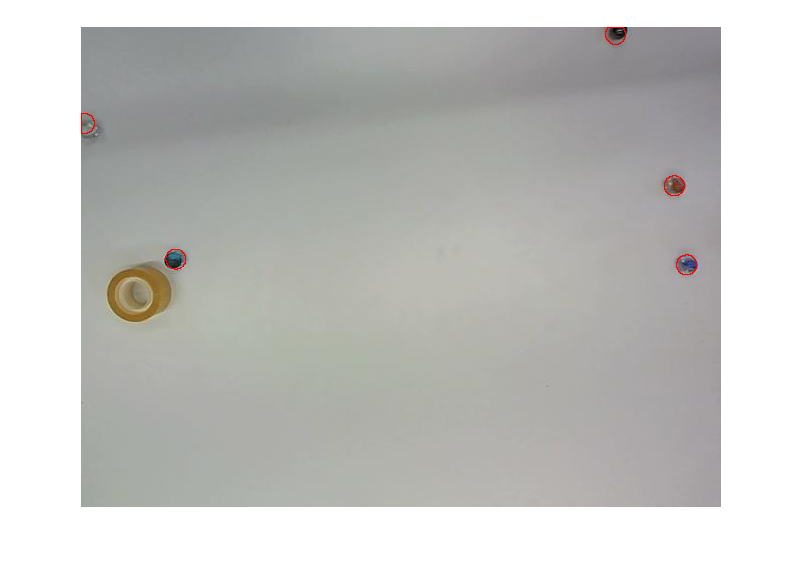
\includegraphics[width=7.5cm]{identification_1.png}
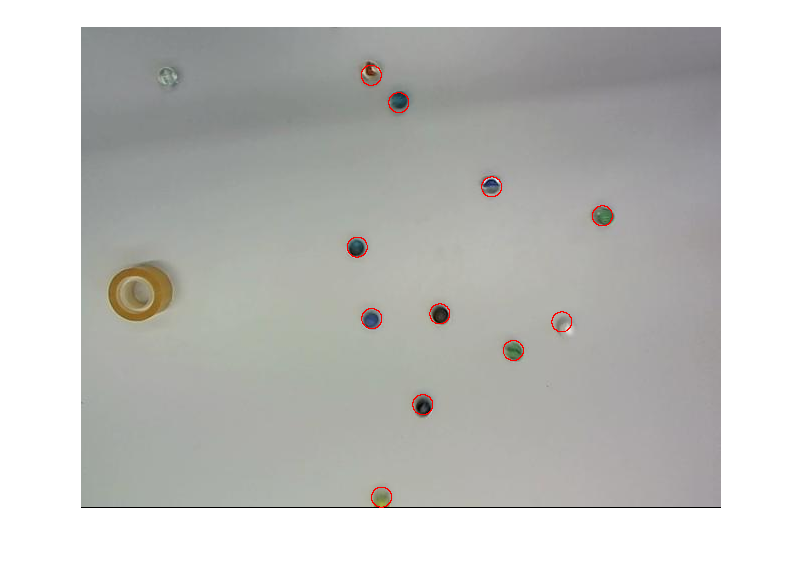
\includegraphics[width=7.5cm]{identification_2.png}
\end{center}

\subsection{Unsuccessful Detections}

The following two images show where our algorithm failing to detect some of the marbles. This most commonly happens when marbles are too close together and end up being treated as one big blob. 

\begin{center}
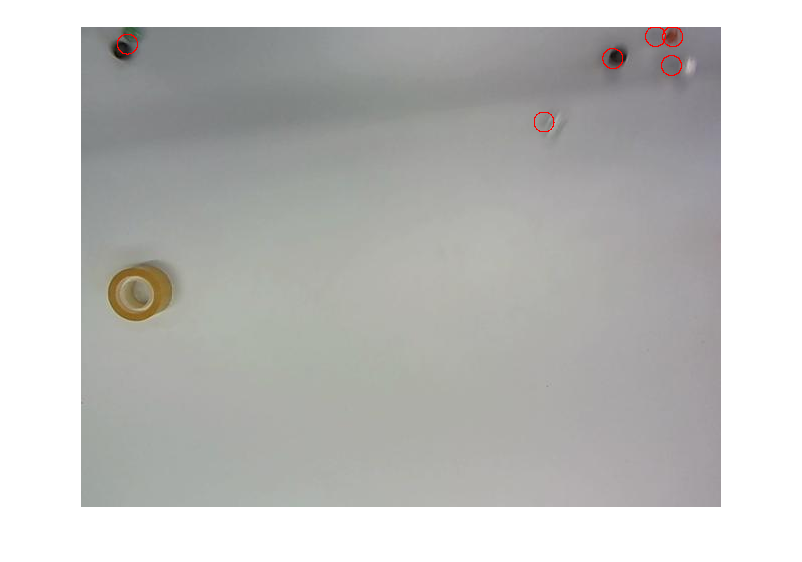
\includegraphics[width=7.5cm]{misidentification_1.png}
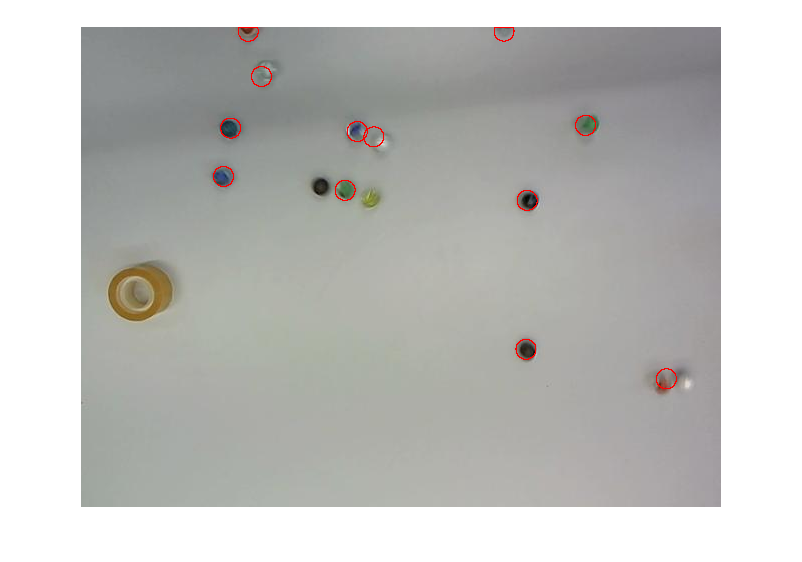
\includegraphics[width=7.5cm]{misidentification_2.png}
\end{center}

In addition, the following two images show that no improvement was gained from performing the blob separation technique. This is mainly attributed to the fact that background subtraction can't remove shadow objects; thus the shadow pixels end up being randomly split between the objects in the blob. This results in an unpredictable shift in the centroids. Two marbles went undetected with blob separation.



\begin{center}
	\begin{figure}[h!]
		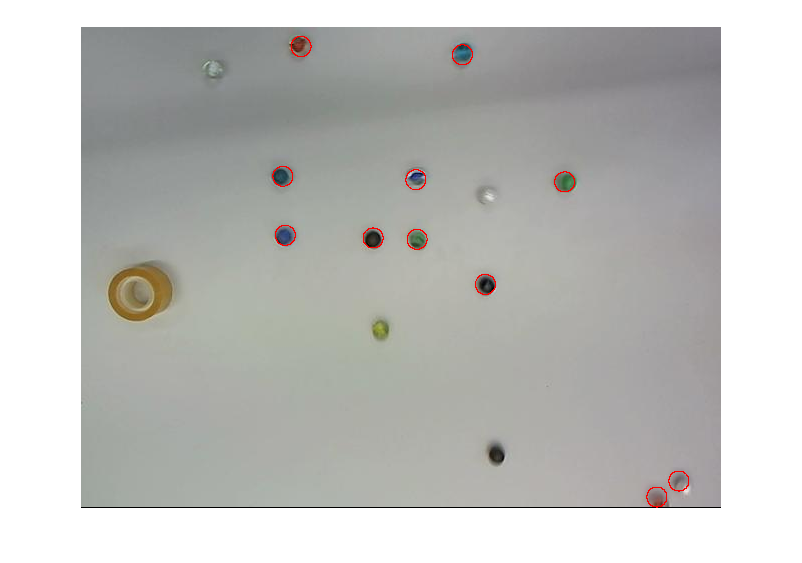
\includegraphics[width=7.5cm]{blob_splitting_with1.png}
		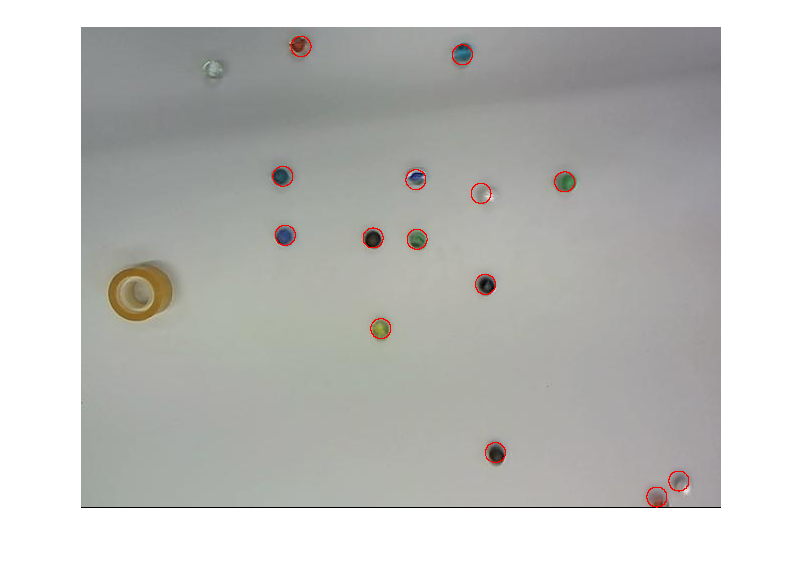
\includegraphics[width=7.5cm]{blop_splitting_without1.png}
		\caption{\textbf{Left:} Marble identification with blob splitting.  \textbf{Right:} Marble identification without blob splitting}
	\end{figure}
\end{center}

\chapter{Marble Tracking}

\section{Algorithm}

Given two consecutive image objects, our marble tracker's main goal is to determine correspondence between the detected marble objects in the new frame and the marble objects in the old frame. In order to make such a decision, we calculated a number of important features for each marble:

\begin{itemize}
\item \textbf{ID:} For any newly detected marble in a frame, it was assigned an id that constitutes the number of the image it was found in and the order at which it was found. Such an id was assigned regardless of any other information about marbles in previous frames.

\item \textbf{Center of Mass:}  Calculated using the connected components property mentioned earlier.

\item \textbf{sumRB:} The sum of the red and blue colour values at the marble's center for the first frame at which it was found. This is one of the two features used to draw correspondence between marbles in consecutive frames.

\item \textbf{colour:} The colour used to show the marble's track .
\end{itemize}

The \textbf{ID} and \textbf{Center of Mass} are calculated when the marbles are first initialized. Given this information for two consecutive frames, we use two features to decide marble correspondence. The first feature is the difference between the sum of the red and blue colour values between the two marbles, and the second feature is the distance between two marbles. Using those two feature, we go through each marble pair in the two frames and assign any two marbles (where the features are below a certain pre-defined threshold) the same \textbf{ID}. Furthermore, the speed feature of any marble was simply the distance travelled between this frame and the previous one.

\section{Performance Analysis}

Despite its simplicity, the algorithm was able to achieve a remarkable performance in tracking the marbles. The only problem we faced was colouring the tracks as some of the marbles in the detection phase were misidentified and caused the tracking algorithm to perform mistakes. For example, two very close marbles were considered one marble in one frame and two marbles in another. This resulted in them being given the same ID. This problem wouldn't have emerged if it wasn't for the algorithm's high dependence on a perfected detection.

We tried to tackle this problem by using blob separation technique mentioned earlier but it resulted in worse results as it over fitted the data and was specific to a certain test frame. Below are two images showing the tracks detected with and without blob separation:

\subsection{Tracking With/Without Blop Separation}

The following images show marble tracking with/without blob separation. Images with blob separation are missing some of the marble tracks, in addition they tend to be more disconnected.

\begin{center}
	\begin{figure}[h!]
		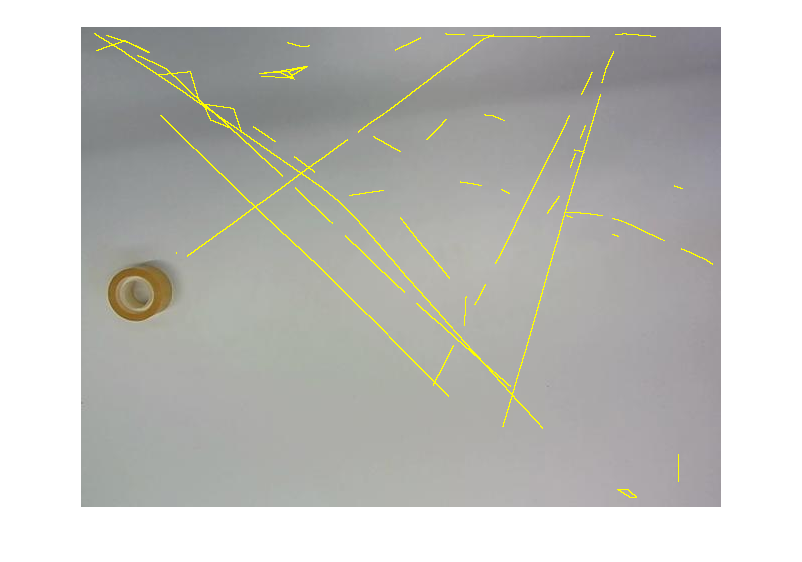
\includegraphics[width=7.5cm]{blob_splitting_track_with2.png}
		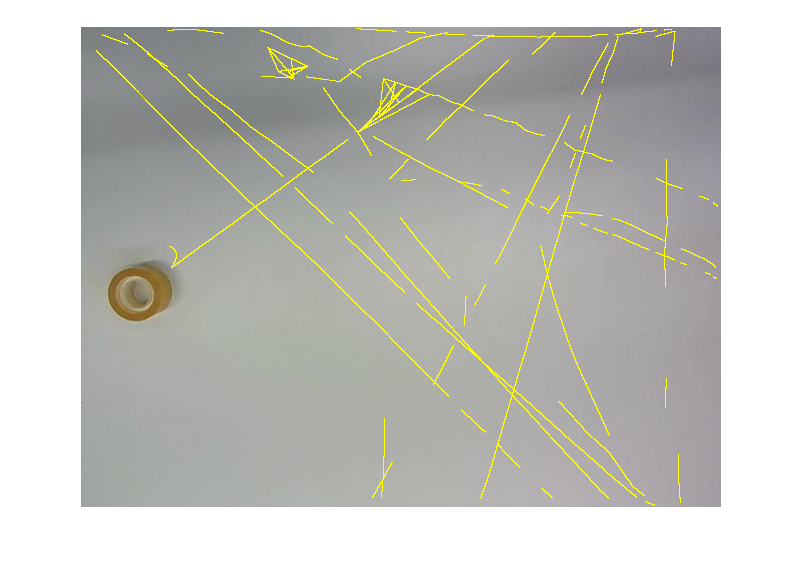
\includegraphics[width=7.5cm]{blob_splitting_track_without2.png}
		\caption{\textbf{Left:} Marble racking with blob splitting.  \textbf{Right:} Marble tracking without blob splitting}
	\end{figure}
\end{center}

\subsection{Final Marble Tracking Result}

The following image shows our final marble tracks using optimum feature values as mentioned before. The disconnection in the marble tracks is caused by misidentified marble correspondences. Nevertheless, most marble tracks were partially identified.

\begin{center}
	\begin{figure}[h!]
		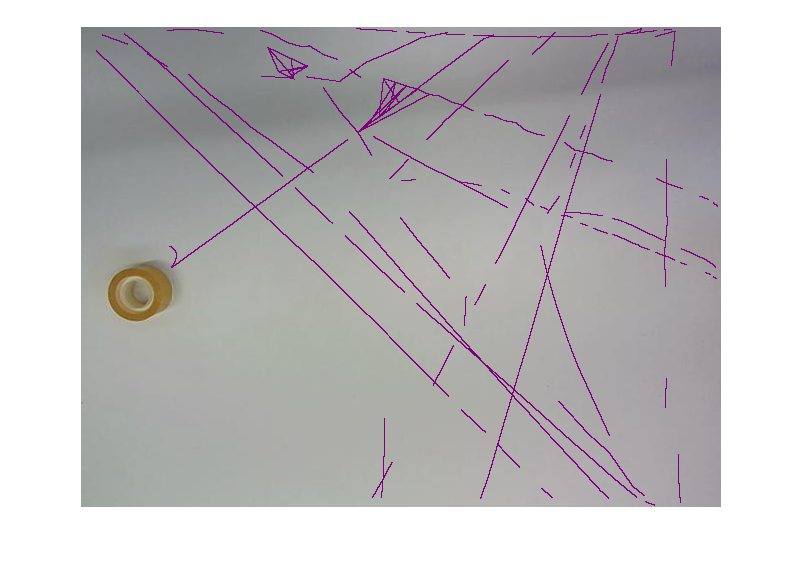
\includegraphics[width=15cm]{track_purple_30diff.png}
	\end{figure}
\end{center}

\chapter{Code Appendix}

\section{Main script}
\begin{lstlisting}
%--------------------------------------------------------------------------
%Workspace clean-up

clc;    %Clear the command window.
close all;  %Close all figures (except those of imtool).
clear;  %Erase all existing variables from workspace.
clearvars; %Remove all stored variables from memory.
clear classes; %Remove all stored class objects.
%--------------------------------------------------------------------------
%Add classes and functions to path
addpath('my_classes', 'my_functions', 'saved_variables');
%--------------------------------------------------------------------------
%DATASET SELECTOR
dataset = 'dataset';

%NUMBER OF IMAGES
num_images = 71;

%TASK SELECTOR
%Select which task you want the code to accomplish:
% 1 --> Marble Detection
% 2 --> Tracking
task = 2;

%DIFFERENCE THRESHOLD
diffThreshold = 40;

%MAX MARBLE CORRESPONDENCE
maxDifference =  30;

%BACKGROUND IMAGE
backgroundImage = myImage();
backgroundImage.dataset = dataset;
backgroundImage.number = 1;
backgroundImage = backgroundImage.generatePath();
backgroundImage = backgroundImage.readImage();

%----------------------------Task 1----------------------------------------
if (task == 1)
    
    track_image = backgroundImage.data;
    
    for imageNum = 1 : num_images
        
        %Initialize target image
        image = myImage();
        image.dataset = dataset;
        image.number = imageNum;
        image = image.generatePath();
        image = image.readImage();

        %Perform background subtraction on image
        image = image.removeBackground(backgroundImage.data, diffThreshold);
        
        %If this is the first image, use it as the previous image in
        %marble tracking
        if (imageNum == 1)
            prevImage = myImage();
            prevImage.dataset = dataset;
            prevImage.number = imageNum;
            prevImage = prevImage.generatePath();
            prevImage = prevImage.readImage();
            prevImage = prevImage.removeBackground(backgroundImage.data, ...
                diffThreshold);
            prevImage = prevImage.identifyMarbles();
        end 
        
        %Identify location of marbles in image
        image = image.identifyMarbles();
        image = image.locateClosestMarble(prevImage, maxDifference);

        %Initialize final image to be labeled and displayed
        finalImage = image.data;

        %Radius of circles to draw around identified marbles
        radius = 10;

        %Draw circles around each of the detected marbles. Radius of each 
        %circle is 10 pixels
        for marble = 1 : size(image.marbles,2)
            
            finalImage = drawCircle(finalImage,image.marbles(marble).com, ...
                radius,'r',1000);
        end

%         for marble = 1 : size(image.marbles,2)
%            display(image.marbles(marble).ID);
%         end
%         subplot(2,2,1), imshow(image.data);
%         subplot(2,2,2), imshow(image.preprocessed);
%         subplot(2,2,3), imshow(image2.preprocessed);
        imshow(finalImage);
        pause(1);
        
        prevImage = image;
    end
end
    
%----------------------------Task 2----------------------------------------
if (task == 2)
    
    %Initialize image to contain track of each marble
    track_image = backgroundImage.data;
    
    %Array of colours
    colours = ['y'];
    
    current_colour = 1;
    
    for imageNum = 1 : num_images
        
        %Initialize target image
        image = myImage();
        image.dataset = dataset;
        image.number = imageNum;
        image = image.generatePath();
        image = image.readImage();

        %Perform background subtraction on image
        image = image.removeBackground(backgroundImage.data, diffThreshold);
        
        %If this is the first image, use it as the previous image in
        %marble tracking
        if (imageNum == 1)
            prevImage = myImage();
            prevImage.dataset = dataset;
            prevImage.number = imageNum;
            prevImage = prevImage.generatePath();
            prevImage = prevImage.readImage();
            prevImage = prevImage.removeBackground(backgroundImage.data, ...
                diffThreshold);
            prevImage = prevImage.identifyMarbles();
        end 
        
        %Identify location of marbles in image
        image = image.identifyMarbles();
        image = image.locateClosestMarble(prevImage, maxDifference);

        %Draw line between marbles identified as having the same ID between
        %frames
        for marble = 1 : size(image.marbles,2)
            for prevMarble = 1 : size(prevImage.marbles,2)
                
                if (image.marbles(marble).ID == prevImage.marbles(prevMarble).ID)
                    
                    if isempty(prevImage.marbles(prevMarble).colour)
                        %Assign marble a coloured track
                        image.marbles(marble).colour = colours(current_colour);
                        %Increment next colour. Start again at zero if we run
                        %out of colours in the array
                        current_colour = mod(current_colour, 1) + 1;
                    end

                    track_image = drawLine(track_image, image.marbles(marble).com, ...
                        prevImage.marbles(prevMarble).com, ...
                        colours(current_colour), 1000);
                end
            end
        end
        
        prevImage = image;
    end
    imshow(track_image);
end
\end{lstlisting}

\section{myImage class}
\begin{lstlisting}
classdef myImage
    %IMAGEHANDLE Class representing individual image frames
%--------------------------------------------------------------------------
    properties
        
        %Dataset to which image belongs
        dataset;
        
        %Image number in the dataset
        number;
        
        %Path to image
        path;
        
        %Pre-defined image height and width
        height = 480;
        width = 640;
        
        %Stores image pixel information in a heightxwidthx3 variable,
        %values are in uint8 format
        data;
        
        %Stores preprocessed version of the image
        preprocessed;
        
        %Background subtracted version of this image
        diff;
        
        %Binary version of the background subtracted image
        binaryDiff;
        
        %Connected components object of this image
        CC;
        
        %Region properties of all the components in the image
        rProps;
        
        %Array containing marble objects currently in the image.
        %Initialized to a pre-defined maximum marbles per image.
        marbles;
    end 
%--------------------------------------------------------------------------    
    methods
        
    function obj = myImage()
    %Class construtor. Avoid requiring initialization parameters for
    %greater flexibility

         obj.marbles = myMarble.empty(18, 0);
    end

    function obj = generatePath(obj)
    %Given a number, this function returns the corrosponding image
    %name. dataset should be the name of the dataset's directory


            %Convert image number to string in preperation for
            %concatination.
            str_number = num2str(obj.number);

            %Generate name for image path
            obj.path = strcat(obj.dataset,'/',str_number,'.jpg');
    end

    function obj = readImage(obj)
    %Reads image information and stores it in this object, returns
    %error if image path not generated yet.

            obj.data = imread(obj.path);
    end

    function obj = removeBackground(obj, background, threshold)
    %Given a background and a threshold, perform background subtraction
    %on this image to obtain the resulting rgb and binary versions.

    [obj.diff, obj.binaryDiff] = sub_background(background, ...
                                    obj.data, threshold);
    end

    function obj = identifyMarbles(obj)
    %Attempts to identify all marbles in this image. Image must have
    %background subtracted versions removed first. Stores list of
    %marble objects in this image. Marbles are given an ID starting
    %with the frame's number as the prefix.

    %for each conencted component, find the center of mass,inialize
    %a marble component, add it to the array marbles.

        %Make sure background subtracted versions of image exist
        if (isempty(obj.diff) || isempty(obj.binaryDiff))
            error('Remove background from image first!');
        else

            %Create disk image structuring with radius 3
            se = strel('disk',4);

            %Apply image open and store in this image's preprocess 
            %variable
            obj.preprocessed = imopen(obj.binaryDiff, se);

            %Find connected components
            obj.CC = bwconncomp(obj.preprocessed);

            %Compute region properties of all marbles
            obj.rProps = regionprops(obj.CC,'Centroid', 'Area', ...
                    'PixelList', 'MajorAxisLength', 'MinorAxisLength');

            %Loop through each connected components, identifying and
            %initializing marble objects
            id = 1; 
            for cc = 1 : size(obj.CC.PixelIdxList, 2)

                % If the ratio of the major axis is a certain ratio
                % higher than the minor axis, then treat this as two
                %marbles
%                     axisRatio = obj.rProps(cc).MajorAxisLength / ...
%                                     obj.rProps(cc).MinorAxisLength;
%                     if axisRatio > 1.35
%                         
%                        %Do histogram.
%                        pixel_list = obj.rProps(cc).PixelList;
%                        [a,~] = size(pixel_list);
%                        bw_img = zeros(obj.height, obj.width);
%                        
%                        for iter = 1 : a
%                            bw_img(pixel_list(iter, 2), pixel_list(iter, 1)) = ...
%                                 sum(obj.data(pixel_list(iter, 2), pixel_list(iter, 1), :)) / 3;
%                        end
%                        
%                        bw_array = reshape(bw_img, obj.height*obj.width, 1);
%                        bw_array(bw_array==0) = [];
%                        first_hist = hist(bw_array, 50);
%                        
%                        filter = gausswin(50, 6);
%                        filter = filter/sum(filter);
%                        smooth_hist = conv(filter,first_hist);
%                        
%                        %Find the valley between the two highest peaks.
%                        inv_hist = 1.01*max(smooth_hist) - smooth_hist;
%                        [~, locsmin] = findpeaks(inv_hist);
%                        
%                        %Distribute points between the peaks.
%                        if (length(locsmin) == 1)
%                            tresh = locsmin;
%                            bin1x = 0;
%                            bin1y = 0;
%                            bin2x = 0;
%                            bin2y = 0;
%                            sum1num = 0;
%                            sum2num = 0;
%                            for iter = 1 : a
%                                aux = sum(obj.data(pixel_list(iter, 2), pixel_list(iter, 1), :)) / 3;
%                                if (aux > tresh)
%                                    sum1num = sum1num + 1;
%                                    bin1x = bin1x  + pixel_list(iter, 2);
%                                    bin1y = bin1y  + pixel_list(iter, 1);
%                                else
%                                    sum2num = sum2num + 1;
%                                    bin2x = bin2x  + pixel_list(iter, 2);
%                                    bin2y = bin2y  + pixel_list(iter, 1);
%                                end 
%                            end
%                            
%                            if (sum1num > 0)
%                                 bin1x = bin1x / sum1num;
%                                 bin1y = bin1y / sum1num;
%                            end
%                            
%                            if (sum2num > 0)
%                                 bin2x = bin2x / sum2num;
%                                 bin2y = bin2y / sum2num;
%                            end
%                           
%                            dist = ((bin2x - bin1x)^2 + (bin2y - bin1y)^2)^0.5;
%                            
%                            if (dist > 8 && sum2num > 0 && sum1num > 0)
%                                marble = myMarble();
%                                marble = marble.assignID((obj.number*100) + id);
%                                marble = marble.assignCOM([bin1y, bin1x]);
%                                marble = marble.calculateSumRB(obj.data);
%                                obj.marbles(id) = marble;
%                                id = id + 1;
% 
%                                marble = myMarble();
%                                marble = marble.assignID((obj.number*100) + id);
%                                marble = marble.assignCOM([bin2y, bin2x]);
%                                marble = marble.calculateSumRB(obj.data);
%                                obj.marbles(id) = marble;
%                                id = id + 1;   
% %                            else
% %                                marble = myMarble();
% %                                marble = marble.assignID((obj.number*100) + id);
% %                                marble = marble.assignCOM([(bin1y+bin2y)/2, (bin1x+bin2x)/2]);
% %                                obj.marbles(id) = marble;
% %                                id = id + 1;
%                            end
%                        end
%                        else
                        %Marble id is the number of the image at which it was
                        %identified concatenated to the order at which it is
                        %identified in a given image
                        marble = myMarble();
                        marble = marble.assignID(obj.number*100 + id);


                        %Assign the center of mass of marble
                        marble = marble.assignCOM(obj.rProps(cc).Centroid);
                        marble = marble.calculateSumRB(obj.data);

                        %Loop through each existant marble object and check for
                        %duplicate ID.
                        for marbleNum = 1 : size(obj.marbles,2)

                            if (marble.ID == obj.marbles(marbleNum).ID)
                                error('Marble with that ID already exists!');
                            end
                        end
                        %Add this marble to our list of detected marbles
                        obj.marbles(id) = marble;
                        id = id + 1;
            end
        end
    end

    function obj = locateClosestMarble(obj, prevImage, maxDifference)
    %Given an image with a detected marbles and this image, the
    %function will attempt to find the corrosponding marble in this
    %image

        %If marbles have been detected in the previous image
        if ~isempty(prevImage.marbles)

            %Loop through each marble in the previous image trying to
            %find its corrospondence in this image
            for marble = 1 : size(obj.marbles,2)

                comMarble = obj.marbles(marble).com;

                for prevMarble = 1 : size(prevImage.marbles,2)

                    comPrevMarble = prevImage.marbles(prevMarble).com;

                    distance = ((comMarble(1) - comPrevMarble(1))^2 + ...
                        (comMarble(2) - comPrevMarble(2))^2)^0.5;

                    if (abs(obj.marbles(marble).sumRB - ...
                            prevImage.marbles(prevMarble).sumRB) ...
                                < maxDifference) && (distance < 35)

                            %Assign this marble the ID of its
                            %correspondence in the previous image
                            obj.marbles(marble).ID = ...
                                prevImage.marbles(prevMarble).ID;

                            %Copy colour used to track previous marble 
                            %to this marble
%                                 obj.marbles(marble).colour = ...
%                                     prevImage.marbles(prevMarble).colour;

                            %Find speed of this marble
                            obj.marbles(marble).speed = distance; 
                    end

                end
            end
        end


    end
end  
end
\end{lstlisting}

\section{myMarble class}
\begin{lstlisting}
classdef myMarble
    %MYMARBLE Class representing an individual marble
%-------------------------------------------------------------------------- 
    properties
        
        %Identification number of marble
        ID;
        
        %Center of mass of the marble
        com;
        
        %2D histogram of the r/g components from normalised RGB values
        histogram;
        
        %Sum of red and blue values in this marble's center
        sumRB;
        
        %Colour used to track marble
        colour;
        
    end
%--------------------------------------------------------------------------    
    methods
        
        
        function obj = myMarble()
        %Class constructor.
        end
        
        function obj = assignID(obj, ID)
        %Assign an ID to this marble
        
            obj.ID = ID;
        end
        
        function obj = assignCOM(obj, com)
        %Assign a center of mass linear coordinate to this marble
            
            obj.com = com;
        end
        
        function obj = calculateSumRB(obj, image)
        %Given an RGB image and this marble with an assigned center of mass
        %calculate the sum of red and green values
        
            marbleX = round(obj.com(1));
            marbleY = round(obj.com(2));
            obj.sumRB = double(image(marbleY, marbleX, 1)) + ...
                            double(image(marbleY, marbleX, 3));
        end
    end
    
end
\end{lstlisting}

\section{subBackground function}
\begin{lstlisting}
function [diffImage, binaryDiffImage] = sub_background(image1, image2, ...
                                            diffThreshold)
%Given two images and a threshold, this function attempts to subtract 
%common pixels from both images, returning the difference image in RGB 
%format and in binary format.
%
%image1 is usually a background image and image2 is the one containing
%objects you are after.
%
%Both images must be of the same size.
   
    %Find image dimensions
    [height, width, depth] = size(image1);
    
    %Find the difference in values between the two images
    diffValues = sum(abs(image1 - image2), 3);
    
	%Matrix to hold resulting background subtracted image
    diffImage = uint8(zeros(height, width, 3));
    binaryDiffImage = zeros(height, width);
    
    %Populate difference matrices
    for iColumn = 1 : width
        for iRow = 1 : height
            
            %If value greater than threshold, that means a non-background
            %object was detected.
            if diffValues(iRow, iColumn) >= diffThreshold
               %Store results in both unit8 format and binary format
               diffImage(iRow, iColumn, :) = ...
                    image2(iRow, iColumn, :);
               binaryDiffImage(iRow, iColumn) = 1;
            end
        end
    end  
end
\end{lstlisting}

\section{rgbnormalize function}
\begin{lstlisting}
function output = rgbnormalize(image_uint)
    %Given an image, this function returns the an rgb normalized version
    %of the image.
 
   image = double(image_uint);
   [H,W,D] = size(image);
   
   %Temporary holder initialized to zeros
   temp = zeros(H,W,D);
   
   %Loop going through every pixel in the image
   for i=1:H
       for j=1:W
           
           %Find average of all colours for
           %that pixel
           csum = image(i,j,1) + image(i,j,2) + image(i,j,3);
           
           temp(i,j,1) = (image(i,j,1) / csum);
           temp(i,j,2) = (image(i,j,2) / csum);
           temp(i,j,3) = (image(i,j,3) / csum);
       end
   end
   output = uint8(temp .* 255);
end
\end{lstlisting}

\section{drawCircle function}
\begin{lstlisting}
function image = drawCircle(image,center,r,color,npoints)
%Function that takes in an RGB image, a 2x1 array representing a center, a
%radius, a colour and a specified number of points, it will produce an
%image with the specified circle superimposed.
%Suggested value for npoints is 100-2000, the more the better!

    %theta value to find all points on the circumference of the circle
    theta=linspace(0,2*pi,npoints);

    %Array containing just the radius value, needed to compute all of the 
    %points
    points = ones(1,npoints) .* r;

    %Find the coordinates that form the circle's circumference
    [X,Y] = pol2cart(theta,points);

    %Adjust all coordinates so that they are consistent with the specified
    %center and round them. Furthermore, change any value that is 0 to 1 to
    %avoid calling a zero or negative index.
    X= round(X+center(1));
    X(X <= 0) = 1;
    Y= round(Y+center(2));
    Y(Y <= 0) = 1;

    %Colour specifier
    colourSpec = zeros(1,3);
    if (color == 'r')
        colourSpec(1,1) = 255;
    end

    %Go through computed XY coordinates, changing them to the specified colour.
    for i=1:npoints
        image(Y(i),X(i),1) = colourSpec(1);
        image(Y(i),X(i),2) = colourSpec(2);
        image(Y(i),X(i),3) = colourSpec(3);
    end
end
\end{lstlisting}

\section{drawLine Function}
\begin{lstlisting}
function image = drawLine(image, point1, point2, color, npoints)
%Function that takes in an RGB image, two 2x1 array representing points
%that need to be connected, a colour and a specified number of points. It 
%will produce an image with the specified circle superimposed.
%Suggested value for npoints is 100-2000, the more the better!

    %Find linear space for x coordinates of the two points
    yLin = linspace(point1(2), point2(2), npoints);
    
    %Find linear space for y coordinate of the two points
    xLin = linspace(point1(1), point2(1), npoints);
    
    %Adjust all coordinates so that they are consistent with the specified
    %center and round them. Furthermore, change any value that is 0 to 1 to
    %avoid calling a zero or negative index.
    xLin = round(xLin);
    xLin(xLin <= 0) = 1;
    yLin= round(yLin);
    yLin(yLin <= 0) = 1;

    %Colour specifier
    colourSpec = zeros(1,3);
    if (color == 'r')
        colourSpec(1,1) = 255;
    elseif (color == 'g')
        colourSpec(1,2) = 255;
    elseif (color == 'b')
        colourSpec(1,3) = 255;
    elseif (color == 'w')
        colourSpec(1,1) = 255;
        colourSpec(1,2) = 255;
        colourSpec(1,3) = 255;
    elseif (color == 'y')
        colourSpec(1,1) = 255;
        colourSpec(1,2) = 255;
    elseif (color == 'p')
        colourSpec(1,1) = 127;
        colourSpec(1,3) = 127;
    elseif (color == 't')
        colourSpec(1,1) = 64;
        colourSpec(1,2) = 224;
        colourSpec(1,3) = 208;
    elseif (color == 'k')
    end
    
    %Go through computed XY coordinates, changing them to the specified colour.
    for i=1:npoints
        image(yLin(i),xLin(i),1) = colourSpec(1);
        image(yLin(i),xLin(i),2) = colourSpec(2);
        image(yLin(i),xLin(i),3) = colourSpec(3);
    end
    
end
\end{lstlisting}

\end{document}